% ============================================================
% Relatório Final de Pesquisa — Programa de Iniciação Científica
% FATEC Baixada Santista "Rubens Lara"
% ============================================================
\documentclass[
    12pt,
    oneside,
    openany,
    a4paper,
    english,
    brazil
]{abntex2}

% ---
% Pacotes básicos
% ---
\usepackage{lmodern}
\usepackage[T1]{fontenc}
\usepackage[utf8]{inputenc}
\usepackage{indentfirst}
\usepackage{color}
\usepackage{graphicx}
\graphicspath{{Images/}}
\usepackage{microtype}
\usepackage{booktabs}
\usepackage{multirow}

% ---
% Matemática — necessário para FTS/lógica fuzzy/prova de teoremas
% ---
\usepackage{amsmath}
\usepackage{amssymb}
\usepackage{amsthm}

\theoremstyle{definition}
\newtheorem{definicao}{Definição}[chapter]

% ---
% Citações no padrão ABNT (NBR 10520)
% ---
\usepackage[brazilian,hyperpageref]{backref}
\usepackage[alf]{abntex2cite}

\renewcommand{\backrefpagesname}{Citado na(s) página(s):~}
\renewcommand{\backref}{}
\renewcommand*{\backrefalt}[4]{%
    \ifcase #1 %
        Nenhuma citação no texto.%
    \or
        Citado na página #2.%
    \else
        Citado #1 vezes nas páginas #2.%
    \fi}%

% ---
% Dados da CAPA e FOLHA DE ROSTO
% ---
\titulo{A Escolha do Modelo como Decisão Axiomática:\\ Misspecification e Fuzzy Time Series}
\autor{Gabriel Gomes}
\local{Santos -- SP}
\data{Agosto/2026}
\orientador[Orientador]{Prof. Dr. Maurício Conceição Mario}
\instituicao{%
    Centro Estadual de Educação Tecnológica Paula Souza
    \par
    Faculdade de Tecnologia da Baixada Santista Rubens Lara
    \par
    Programa de Iniciação Científica}
\tipotrabalho{Relatório final de pesquisa}
\preambulo{Relatório final de pesquisa apresentado à Faculdade de
Tecnologia da Baixada Santista ``Rubens Lara'', do Curso Superior de
Tecnologia em Ciência de Dados, para aprovação no Programa de
Iniciação Científica.}

% ---
% PDF metadata
% ---
\makeatletter
\hypersetup{
    pdftitle={\@title},
    pdfauthor={\@author},
    pdfsubject={\imprimirpreambulo},
    pdfcreator={LaTeX com abnTeX2},
    colorlinks=true,
    linkcolor=black,
    citecolor=black,
    filecolor=black,
    urlcolor=black,
    bookmarksdepth=4
}
\makeatother

\begin{document}

\selectlanguage{brazil}
\frenchspacing

% ============================================================
% ELEMENTOS PRÉ-TEXTUAIS
% ============================================================

\imprimircapa
\imprimirfolhaderosto*

% --- Resumo ---
\setlength{\absparsep}{18pt}
\begin{resumo}
No campo da estatística, modelos estocásticos empregados na previsão de séries temporais constituem ferramentas formais capazes de inferência. Argumenta-se, porém, que a escolha de um modelo de previsão não é uma decisão puramente técnica, mas axiomática, à luz das premissas formais que cada modelo carrega. Esta pesquisa parte da constatação de que a auditoria dessas premissas é frequentemente negligenciada na prática aplicada. O caso motivador é o trabalho de Santos, Campos e Correa (2023), que aplicam doze regressões lineares simples à série de movimentação de carga do Porto de Santos (2005--2022), justificando a escolha pela simplicidade e pelo baixo custo computacional, sem auditar os resíduos. Realizou-se uma bateria de testes de \textit{misspecification} sobre o modelo original (Durbin-Watson, Ljung-Box, Breusch-Pagan, Shapiro-Wilk, Jarque-Bera), demonstrando violação robusta de independência e homocedasticidade. Em seguida, aplicou-se o modelo de Fuzzy Time Series de Chen (1996) aos mesmos dados, com diferenciação para remoção de tendência e reconstrução dos valores em nível. Com base em Mayo, Spanos, da Costa e Krause, articulou-se o conceito de \textit{honestidade axiomática} --- critério normativo segundo o qual um modelo é honesto quando nenhuma afirmação inferencial que dele se extrai excede o que suas premissas formais autorizam. Demonstrou-se que adequação estatística e honestidade axiomática são eixos logicamente independentes, e que o FTS de Chen ilustra honestidade sem que a pergunta de adequação probabilística sequer se aplique a ele.

    \vspace{\onelineskip}
    \noindent
    \textbf{Palavras-chave}: honestidade axiomática; séries temporais fuzzy; misspecification; adequação estatística; filosofia da ciência.
\end{resumo}

\begin{resumo}[Abstract]
    \begin{otherlanguage*}{english}
In statistics, stochastic models used in time series forecasting constitute formal tools capable of inference. We argue, however, that the choice of a forecasting model is not merely technical but axiomatic, given the formal assumptions every model carries. This research stems from the observation that the audit of such assumptions is frequently neglected in applied practice. The motivating case is Santos, Campos, and Correa (2023), who apply twelve simple linear regressions to the Port of Santos cargo movement series (2005--2022), justifying their choice by simplicity and low computational cost, without auditing residuals. A battery of misspecification tests was applied to the original model (Durbin-Watson, Ljung-Box, Breusch-Pagan, Shapiro-Wilk, Jarque-Bera), demonstrating robust violations of independence and homoscedasticity. Subsequently, Chen's (1996) Fuzzy Time Series model was applied to the same data, with differencing to remove trend and reconstruction of level values. Drawing on Mayo, Spanos, da Costa, and Krause, the concept of \textit{axiomatic honesty} was articulated --- a normative criterion according to which a model is honest when no inferential claim extracted from it exceeds what its formal assumptions authorize. It was demonstrated that statistical adequacy and axiomatic honesty are logically independent axes, and that Chen's FTS illustrates honesty without the question of probabilistic adequacy even applying to it.

        \vspace{\onelineskip}
        \noindent
        \textbf{Keywords}: axiomatic honesty; fuzzy time series; misspecification; statistical adequacy; philosophy of science.
    \end{otherlanguage*}
\end{resumo}

% --- Listas ---
\pdfbookmark[0]{\listfigurename}{lof}
\listoffigures*
\cleardoublepage

\pdfbookmark[0]{\listtablename}{lot}
\listoftables*
\cleardoublepage

\begin{siglas}
    \item[ABNT] Associação Brasileira de Normas Técnicas
    \item[BENT] Bad Evidence, No Test
    \item[BLUE] Best Linear Unbiased Estimator
    \item[FATEC BS] Faculdade de Tecnologia da Baixada Santista
    \item[FLR] Fuzzy Logic Relationship (Relação Lógica Fuzzy)
    \item[FLRG] Fuzzy Logic Relationship Group (Grupo de Relações Lógicas Fuzzy)
    \item[FTS] Fuzzy Time Series (Séries Temporais Fuzzy)
    \item[IC] Iniciação Científica
    \item[LRM] Linear Regression Model
    \item[M-S] Misspecification (Má Especificação)
    \item[NIID] Normal, Independente e Identicamente Distribuído
    \item[OLS] Ordinary Least Squares (Mínimos Quadrados Ordinários)
    \item[PIC] Programa de Iniciação Científica
    \item[PWFTS] Probabilistic Weighted Fuzzy Time Series
\end{siglas}

\pdfbookmark[0]{\contentsname}{toc}
\tableofcontents*
\cleardoublepage

% ============================================================
% ELEMENTOS TEXTUAIS
% ============================================================
\textual

% ============================================================
\chapter{Introdução}
\label{cap:introducao}
% ============================================================

A aplicação de modelos estatísticos à previsão de séries temporais é prática consolidada em ciência de dados, econometria e engenharia. No entanto, a escolha de um modelo de previsão raramente é reconhecida como o que, do ponto de vista lógico-formal, ela efetivamente é: uma \textbf{decisão axiomática}. Todo modelo estatístico --- seja ele uma regressão linear, um processo ARIMA ou um modelo de Séries Temporais Fuzzy --- opera dentro de um sistema axiomático específico, carregando premissas formais que delimitam o alcance legítimo de suas inferências.

Esta pesquisa nasce da constatação de que a auditoria dessas premissas é frequentemente negligenciada na prática aplicada, mesmo em produção científica formalmente revisada. Conforme documentam \citeonline{mayo2004methodology}, a crescente disponibilidade de poder computacional e \textit{software} estatístico aumentou a facilidade com que profissionais aplicam métodos estatísticos, mas isso não foi acompanhado por atenção à verificação das premissas nas quais esses métodos se baseiam. \citeonline{nielsen2020practical} confirma esse padrão ao dedicar uma seção inteira de seu livro à pergunta ``\textit{Why Not Use a Linear Regression?}'', reconhecendo que ``\textit{real-world analysts take liberties with model assumptions from time to time}'' --- prática legítima apenas quando \textbf{consciente} das potenciais consequências.

O caso motivador desta pesquisa é o trabalho de \citeonline{santos2023porto}, que aplica doze regressões lineares simples --- uma para cada mês, como estratégia para mitigar sazonalidade --- à série temporal de movimentação de carga do Porto de Santos (2005--2022). Os autores justificam a escolha pela simplicidade e pelo baixo custo computacional frente ao SARIMA, sem nunca auditar os resíduos do modelo. Os altos coeficientes de determinação ($R^2 \geq 80\%$) são apresentados como evidência de sucesso.

A partir desse caso, articulou-se o conceito central desta pesquisa: a \textbf{honestidade axiomática}, critério normativo que distingue modelos que respeitam os limites inferenciais impostos por suas próprias premissas daqueles que os ultrapassam sem verificação. Para demonstrar esse conceito em operação, aplicou-se o modelo de Fuzzy Time Series de \citeonline{chen1996forecasting} aos mesmos dados, ilustrando como um modelo pode ser honesto sem que a pergunta de adequação probabilística sequer se aplique a ele.

% ============================================================
\section{Justificativa do Tema}
\label{sec:justificativa}
% ============================================================

A relevância desta pesquisa situa-se na interseção entre ciência de dados e filosofia da ciência. No âmbito da formação em Ciência de Dados, a auditoria de pressupostos estatísticos é um tema transversal a todas as disciplinas quantitativas, mas raramente é abordada como questão \textit{lógico-formal}. A distinção entre um modelo que falha em seus próprios termos e um que opera sob um sistema axiomático diferente é fundamental para a prática profissional responsável.

Ademais, a teoria de conjuntos fuzzy \cite{zadeh1965fuzzy} e seus desdobramentos em séries temporais \cite{song1993fuzzy, chen1996forecasting} representam uma alternativa legítima dentro de um arcabouço lógico não clássico, cuja fundamentação metamatemática foi estabelecida por \citeonline{hajek1998metamathematics}. A pesquisa conecta, portanto, dois domínios que raramente dialogam: a prática de modelagem em séries temporais e a reflexão filosófica sobre o que constitui uma aplicação legítima de um modelo formal.

% ============================================================
\section{Problema da Pesquisa}
\label{sec:problema}
% ============================================================

Em que sentido a escolha de um modelo estatístico constitui uma decisão axiomática, e como essa dimensão pode ser auditada e comparada entre sistemas formais distintos --- probabilístico clássico e lógica fuzzy?

% ============================================================
\subsection{Hipóteses ou Suposições}
\label{subsec:hipoteses}
% ============================================================

A hipótese central desta pesquisa é que um modelo pode ser simultaneamente \textbf{inadequado} (suas premissas não valem para os dados) e \textbf{desonesto} (afirma inferências que excedem o que foi verificado) --- e que essas são propriedades logicamente independentes, não sinônimas. A regressão linear de \citeonline{santos2023porto} constitui, hipoteticamente, um exemplo de ambas ao mesmo tempo; um modelo de Fuzzy Time Series aplicado aos mesmos dados pode ser honesto sem que a pergunta de adequação (no sentido probabilístico) sequer se aplique a ele.

% ============================================================
\section{Objetivos}
\label{sec:objetivos}
% ============================================================

% ============================================================
\subsection{Objetivo Geral}
\label{subsec:objetivo-geral}
% ============================================================

Investigar a escolha de modelos de previsão para séries temporais como uma decisão axiomática, auditando o caso de \citeonline{santos2023porto} e propondo uma alternativa baseada em Fuzzy Time Series como ilustração de honestidade axiomática.

% ============================================================
\subsection{Objetivos Específicos}
\label{subsec:objetivos-especificos}
% ============================================================

\begin{enumerate}
    \item Auditar estatisticamente o modelo de regressão linear de \citeonline{santos2023porto} mediante testes de \textit{misspecification} (Durbin-Watson, Ljung-Box, Breusch-Pagan, Shapiro-Wilk, Jarque-Bera).
    \item Aplicar o modelo de Fuzzy Time Series de \citeonline{chen1996forecasting} aos mesmos dados do Porto de Santos, removendo a tendência por diferenciação e reconstruindo os valores em nível por soma acumulada.
    \item Articular, com base em \citeonline{mayo2018statistical}, \citeonline{spanos2007curve}, \citeonline{dacosta1994sistemas} e \citeonline{krause2022models}, o conceito de \textit{honestidade axiomática} como critério normativo independente da adequação estatística.
    \item Demonstrar, por meio da comparação dos modelos, que adequação (relação modelo--dados) e honestidade (relação afirmação--auditoria) são eixos logicamente distintos.
\end{enumerate}

% ============================================================
\chapter{Referencial Teórico}
\label{cap:referencial}
% ============================================================

% ============================================================
\section{Regressão Espúria e o Problema da Má Especificação}
\label{sec:regressao-espuria}
% ============================================================

O fenômeno da regressão espúria, demonstrado por \citeonline{granger1974spurious}, constitui o ponto de partida econométrico desta pesquisa. Os autores demonstram, via simulação de Monte Carlo, que regredir dois \textit{random walks} independentes produz rejeição espúria de $H_0$ (ausência de relação) em aproximadamente 75\% das simulações ao nível de significância de 5\%. O diagnóstico oferecido é direto: $R^2$ alto acompanhado de estatística Durbin-Watson baixa não constitui evidência de relação real --- ``\textit{a única conclusão possível é que a equação está mal-especificada, qualquer que seja o valor de $R^2$}'' \cite[p.~117]{granger1974spurious}.

\citeonline{mayo2004methodology} refinam essa problemática ao distinguir dois níveis de perguntas em qualquer modelo estatístico. A \textbf{questão primária} (``dado que o modelo é válido, quão bom preditor é $x$?'') --- respondida por $R^2$, $p$-valores e coeficientes --- só é interpretável se precedida pela \textbf{questão secundária} (``as premissas probabilísticas do modelo realmente valem para os dados?''), que exige testes realizados \textit{fora} do modelo. Os autores identificam cinco pressupostos do modelo de regressão linear: normalidade, linearidade, homocedasticidade, independência e invariância temporal. A passagem ``\textit{statistical adequacy is tantamount to the claim that data $y_0$ constitute a `truly typical realization' of the stochastic mechanism described by $M_v(y)$}'' \cite[p.~1020]{mayo2004methodology} sintetiza o critério de adequação estatística adotado nesta pesquisa.

\citeonline{spanos2007curve} aprofunda a distinção ao opor dois paradigmas de avaliação de modelos: a \textbf{aproximação matemática} (cujo critério é a qualidade do ajuste, \textit{goodness-of-fit}, medida por $R^2$) e a \textbf{modelagem estatística} (cujo critério é a adequação estatística, verificada pela não-sistematicidade dos resíduos). O estudo de caso Kepler \textit{versus} Ptolomeu é ilustrativo: ambos os modelos apresentam $R^2$ excelente (0,999 e 0,992, respectivamente), mas apenas o modelo de Kepler passa nos cinco testes de \textit{misspecification} (todos $p > 0{,}10$); o modelo de Ptolomeu falha em todos ($p \approx 0{,}00000$).

% ============================================================
\section{Teste Severo e o Princípio BENT}
\label{sec:teste-severo}
% ============================================================

\citeonline{mayo2018statistical} propõe que uma inferência estatística é bem sustentada apenas se o procedimento que a gerou \textit{provavelmente teria detectado a falha}, caso a hipótese fosse falsa. Esse é o critério do \textbf{teste severo}. Complementarmente, a autora formula o princípio BENT (\textit{Bad Evidence, No Test}): se os dados $x$ concordam com uma alegação $C$, mas o método empregado tinha pouca ou nenhuma capacidade de detectar falhas em $C$ mesmo que existissem, então o resultado configura ``má evidência, sem teste'' \cite[§1.1]{mayo2018statistical}.

Aplicado ao caso de \citeonline{santos2023porto}, o diagnóstico é direto: a afirmação de sucesso do modelo com base em $R^2 \geq 80\%$ sem qualquer verificação das premissas subjacentes configura precisamente um BENT --- os dados concordam com o modelo (ajuste visual razoável), mas o procedimento não testou se as condições para que essa concordância seja evidência legítima de fato valem.

% ============================================================
\section{Pluralismo Lógico e Sistemas Formais}
\label{sec:pluralismo}
% ============================================================

A passagem do paradigma probabilístico clássico para o paradigma fuzzy exige uma fundamentação filosófica que justifique a legitimidade de se operar com lógicas alternativas. \citeonline{dacosta1994sistemas} e \citeonline{dacosta1980ensaio} fornecem essa fundamentação ao defender que existem diversas lógicas legítimas, cada uma adequada a problemas específicos, sem que nenhuma seja ``a lógica verdadeira'' de forma absoluta --- posição denominada \textbf{pluralismo lógico}. Da Costa traça uma analogia explícita entre a relação geometria euclidiana/não-euclidiana e a relação lógica clássica/lógicas alternativas, argumentando que, assim como a geometria não-euclidiana não ``invalida'' a euclidiana mas constitui um sistema formal distinto com domínios de aplicação próprios, lógicas não clássicas (paraconsistentes, fuzzy, intuicionistas) são formalismos legítimos, não ``desvios'' de uma norma.

\citeonline{krause2017logical} demonstram que todo modelo ou teoria científica se baseia em uma \textbf{espécie de estrutura} (\textit{species of structure}) no sentido de Bourbaki --- um conjunto de conjuntos-base sujeitos a axiomas. \citeonline{krause2022models} reforça esta posição ao afirmar que ``\textit{the use of models of scientific theories should not be done without qualifications about the mathematics being used to build the models}'' \cite[p.~39]{krause2022models}. A distinção é essencial para esta pesquisa: a regressão linear de \citeonline{santos2023porto} opera sobre a espécie de estrutura dos axiomas de Kolmogorov e do modelo NIID (Normal, Independente e Identicamente Distribuído); o modelo de Fuzzy Time Series opera sobre a espécie de estrutura da teoria de conjuntos fuzzy de \citeonline{zadeh1965fuzzy}. São sistemas formais distintos, com premissas distintas, e portanto com critérios de verificação distintos.

É importante distinguir três sentidos da palavra ``modelo'' que atravessam esta pesquisa: (i) o sentido \textbf{lógico/metamatemático}, no qual modelo é uma estrutura que satisfaz um conjunto de axiomas (Tarski, Suppes, van Fraassen); (ii) o sentido \textbf{estatístico}, no qual modelo é uma família de distribuições parametrizada (Mayo, Spanos); e (iii) o sentido \textbf{aplicado}, no qual modelo é um algoritmo específico (Chen FTS, OLS). Esses três sentidos são usados nesta pesquisa de forma complementar, e a confusão entre eles é, ela mesma, uma fonte potencial de equivocação.

% ============================================================
\section{Séries Temporais Fuzzy: Fundamentos}
\label{sec:fts}
% ============================================================

A teoria de conjuntos fuzzy, introduzida por \citeonline{zadeh1965fuzzy}, estende a teoria clássica de conjuntos ao permitir graus de pertinência no intervalo $[0,1]$, em contraste com a pertinência binária $\{0,1\}$ da lógica bivalente. \citeonline{hajek1998metamathematics} estabeleceu a fundamentação metamatemática dessa teoria, demonstrando que o raciocínio aproximado possui bases matemáticas sólidas, com sintaxe, semântica e completude bem definidas, consolidadas sobre lógicas polivalentes infinitas baseadas em \textit{t-normas}.

A partir dessa base, \citeonline{song1993fuzzy} introduzem as \textbf{Séries Temporais Fuzzy} (FTS), motivados pela necessidade de modelar variáveis linguísticas como função do tempo, deslocando-se dos modelos estocásticos bivalentes para a teoria de conjuntos fuzzy. O modelo original de Song e Chissom, contudo, envolvia operações matriciais de alto custo computacional. \citeonline{chen1996forecasting} propõe uma simplificação fundamental: substituir as operações matriciais por operações aritméticas simples, mediante a formulação de \textit{Fuzzy Logic Relationships} (FLR) e \textit{Fuzzy Logic Relationship Groups} (FLRG), com defuzzificação pela média dos pontos médios:

\begin{equation}
\hat{y}_{t+1} = \frac{1}{p}\sum_{k=1}^{p} m_k
\label{eq:chen}
\end{equation}

\noindent onde $m_k$ é o ponto médio do $k$-ésimo conjunto fuzzy consequente e $p$ é o número de consequentes no FLRG ativado.

O método de Chen envolve as seguintes etapas: (i) definição do universo de discurso e do número de partições; (ii) criação dos conjuntos fuzzy para cada partição; (iii) fuzzificação da série temporal $Y(t)$ em uma FTS $F(t)$; (iv) formulação das FLRs e agrupamento em FLRGs; e (v) defuzzificação para gerar previsões numéricas.

Desenvolvimentos recentes incluem o PWFTS (\textit{Probabilistic Weighted Fuzzy Time Series}) de \citeonline{silva2019pwfts}, que incorpora pesos probabilísticos às transições entre estados fuzzy, e o tutorial de \citeonline{lucas2021tutorial}, que sistematiza os avanços e desafios da área.

% ============================================================
\chapter{Procedimentos Metodológicos}
\label{cap:metodologia}
% ============================================================

Esta pesquisa adota uma abordagem \textbf{exploratória e comparativa}, combinando análise quantitativa (testes estatísticos e aplicação de modelos) com reflexão teórico-filosófica (articulação do conceito de honestidade axiomática). A classificação segue \citeonline{gil2017elaborar}: quanto à natureza, trata-se de pesquisa aplicada; quanto aos objetivos, exploratória; quanto à abordagem, predominantemente quantitativa com componente qualitativo na discussão filosófica; quanto aos procedimentos, pesquisa bibliográfica associada a experimentação computacional.

% ============================================================
\section{Dados}
\label{sec:dados}
% ============================================================

Utilizou-se a série temporal de movimentação de carga mensal do Porto de Santos, período de janeiro de 2005 a dezembro de 2022, totalizando 216 observações. A base é a mesma empregada por \citeonline{santos2023porto}, obtida da Autoridade Portuária de Santos. O período de treinamento compreende janeiro de 2005 a dezembro de 2022 (216 observações para a auditoria \textit{in-sample} da regressão linear) e o período de teste (previsão \textit{out-of-sample}) compreende janeiro de 2023 a março de 2026 (39 observações).

A análise exploratória revelou três componentes na série: (i) \textbf{tendência} crescente ao longo do período; (ii) \textbf{sazonalidade} anual pronunciada, com picos e vales recorrentes; e (iii) \textbf{resíduo} (componente irregular). A decomposição STL (\textit{Seasonal and Trend decomposition using Loess}), apresentada na Figura~\ref{fig:stl}, confirmou visualmente esses componentes. Os testes de estacionariedade (ADF e KPSS) indicaram não-estacionariedade da série em nível, com estacionariedade atingida após diferenciação.

\begin{figure}[htb]
\centering
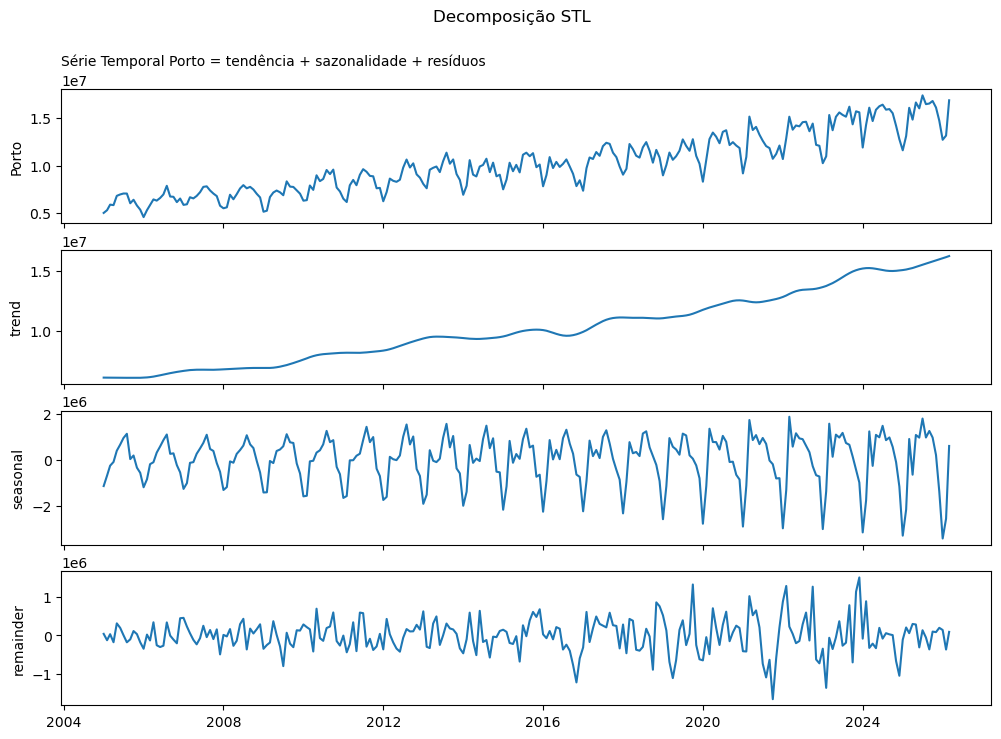
\includegraphics[width=0.85\textwidth]{STL_porto.png}
\caption{Decomposição STL da série temporal do Porto de Santos (período = 12 meses).}
\label{fig:stl}
\end{figure}

% ============================================================
\section{Etapa 1: Auditoria do Modelo de Santos et al. (2023)}
\label{sec:auditoria}
% ============================================================

Reproduziu-se a especificação dos autores: doze regressões lineares simples independentes, uma para cada mês, com o ano como variável independente e a movimentação de carga como variável dependente. Sobre os resíduos agregados, aplicou-se a seguinte bateria de testes de \textit{misspecification}, conforme o protocolo de \citeonline{mayo2004methodology}:

\begin{itemize}
    \item \textbf{Durbin-Watson}: autocorrelação de defasagem 1;
    \item \textbf{Ljung-Box}: autocorrelação conjunta, defasagens 12 e 24;
    \item \textbf{Breusch-Pagan}: heterocedasticidade;
    \item \textbf{Shapiro-Wilk}: normalidade dos resíduos;
    \item \textbf{Jarque-Bera}: normalidade dos resíduos (teste alternativo, baseado em assimetria e curtose).
\end{itemize}

A linearidade nos parâmetros foi tratada como especificação do modelo, não como hipótese testável empiricamente da mesma forma que as demais.

% ============================================================
\section{Etapa 2: Aplicação do Modelo de Fuzzy Time Series}
\label{sec:fts-aplicacao}
% ============================================================

Aplicou-se o modelo de Chen \cite{chen1996forecasting} utilizando a biblioteca pyFTS \cite{silva2018probabilistic} em Python. Dado que o método de Chen assume série estacionária (sem tendência), a série original foi diferenciada ($\Delta y_t = y_t - y_{t-1}$) para remoção da tendência, e o modelo foi aplicado à série diferenciada, com 10 partições triangulares do universo de discurso e FTS de primeira ordem. A avaliação foi realizada por validação \textit{walk-forward} com janela deslizante de 1 passo à frente, ao longo de 39 meses. Os valores em nível foram reconstruídos por soma acumulada das variações previstas.

Adicionalmente, aplicou-se o modelo PWFTS (\textit{Probabilistic Weighted Fuzzy Time Series}) de ordem 3, com 34 partições e diferenciação sazonal de 12 períodos ($\Delta_{12} y_t = y_t - y_{t-12}$), gerando 1.275 regras lógicas fuzzy ponderadas probabilisticamente. A diferenciação sazonal visa capturar o padrão sazonal que o Chen de primeira ordem sobre $\Delta y$ (diferença simples) não contempla --- dado que o domínio original de Song e Chissom (matrículas universitárias) não apresentava sazonalidade.

Para contextualização dentro do paradigma clássico, aplicaram-se também: Holt-Winters aditivo (como exemplo de modelo clássico axiomaticamente alinhado com os dados) e Holt-Winters multiplicativo (como contraexemplo intra-paradigma, demonstrando que a desonestidade não é exclusiva de modelos ``simples'' nem da regressão linear).

% ============================================================
\chapter{Resultados}
\label{cap:resultados}
% ============================================================

% ============================================================
\section{Auditoria da Regressão Linear de Santos et al. (2023)}
\label{sec:resultados-auditoria}
% ============================================================

A Figura~\ref{fig:real-rl} apresenta a série original e o ajuste das doze regressões lineares. A Tabela~\ref{tab:ms-tests} apresenta os resultados da bateria de testes de \textit{misspecification} aplicada aos resíduos.

\begin{figure}[htb]
\centering
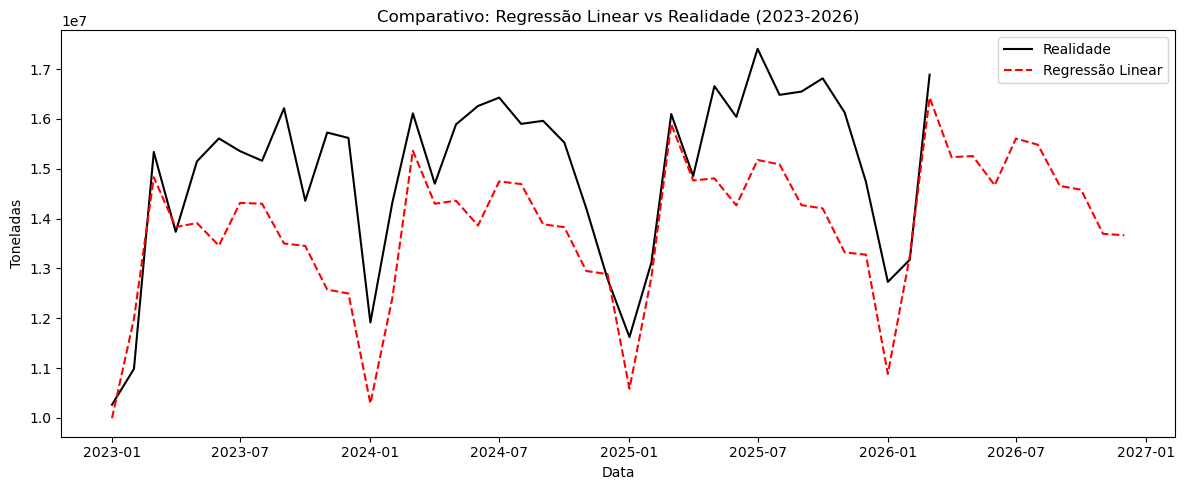
\includegraphics[width=0.85\textwidth]{real_rl.png}
\caption{Série temporal do Porto de Santos (2005--2022) e ajuste das 12 regressões lineares de \citeonline{santos2023porto}.}
\label{fig:real-rl}
\end{figure}

\begin{table}[htb]
\centering
\caption{Testes de \textit{misspecification} sobre os resíduos da regressão linear de \citeonline{santos2023porto}.}
\label{tab:ms-tests}
\begin{tabular}{l c c l}
\toprule
\textbf{Teste} & \textbf{Estatística} & \textbf{Valor-$p$} & \textbf{Veredito} \\
\midrule
Durbin-Watson         & $DW = 0{,}9133$ & ---                              & Autocorrelação positiva forte \\
Ljung-Box (12 lags)   & $LB_{12} = 119{,}27$ & $8{,}63 \times 10^{-20}$   & Rejeita independência \\
Ljung-Box (24 lags)   & $LB_{24} = 135{,}41$ & $1{,}61 \times 10^{-17}$   & Confirma, robusto \\
Breusch-Pagan         & $LM = 19{,}01$       & $1{,}30 \times 10^{-5}$    & Rejeita homocedasticidade \\
Shapiro-Wilk          & $W = 0{,}9873$       & $0{,}051$                  & Não rejeita normalidade \\
Jarque-Bera           & $JB = 7{,}11$        & $0{,}0285$                 & Rejeita normalidade \\
\bottomrule
\end{tabular}
\end{table}

O modelo viola, de forma robusta e estatisticamente decisiva, duas condições de Gauss-Markov: \textbf{independência} (Durbin-Watson e Ljung-Box convergem) e \textbf{homocedasticidade} (Breusch-Pagan, $p = 1{,}30 \times 10^{-5}$). Isso significa que o estimador OLS sequer é BLUE (\textit{Best Linear Unbiased Estimator}) para esses dados, independentemente da questão de normalidade.

Quanto à normalidade, há divergência entre os testes: Shapiro-Wilk não rejeita ($p = 0{,}051$, na fronteira), enquanto Jarque-Bera rejeita ($p = 0{,}0285$). Essa divergência é reportada tal como observada, sem escolher o teste que produz a resposta mais conveniente --- o que seria, em si, um exemplo de desonestidade no sentido definido nesta pesquisa.

A Figura~\ref{fig:diag-rl} apresenta o painel diagnóstico dos resíduos, e a Figura~\ref{fig:resid-rl} exibe o correlograma dos resíduos agregados, evidenciando o padrão de autocorrelação serial.

\begin{figure}[htb]
\centering
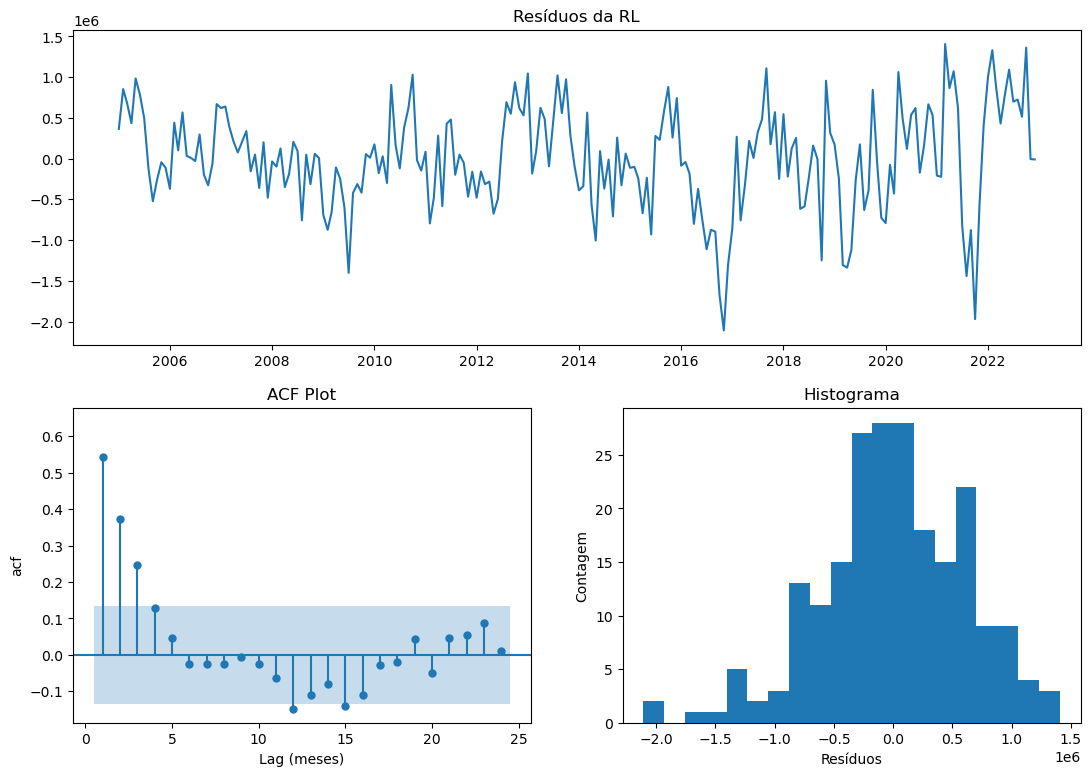
\includegraphics[width=0.85\textwidth]{diag_rl.png}
\caption{Painel diagnóstico dos resíduos da regressão linear de \citeonline{santos2023porto}.}
\label{fig:diag-rl}
\end{figure}

\begin{figure}[htb]
\centering
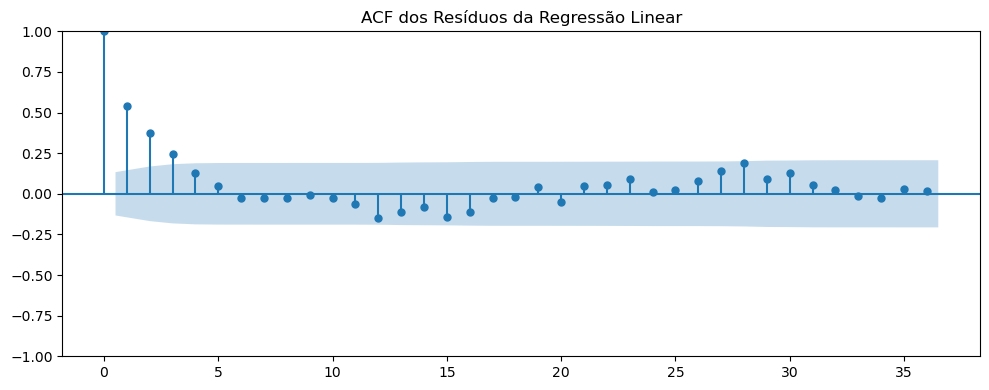
\includegraphics[width=0.7\textwidth]{resid_rl.png}
\caption{Correlograma (ACF) dos resíduos agregados da regressão linear.}
\label{fig:resid-rl}
\end{figure}

% ============================================================
\section{Modelos de Previsão: Diagnóstico Comparado}
\label{sec:resultados-modelos}
% ============================================================

A Tabela~\ref{tab:ljungbox-all} apresenta os resultados do teste de Ljung-Box aplicado aos resíduos de cada modelo, em múltiplas defasagens.

\begin{table}[htb]
\centering
\caption{Teste de Ljung-Box ($p$-valores) sobre resíduos de cada modelo.}
\label{tab:ljungbox-all}
\begin{tabular}{l c c c c l}
\toprule
\textbf{Modelo} & \textbf{Lag 1} & \textbf{Lag 6} & \textbf{Lag 12} & \textbf{Lag 24} & \textbf{Veredito} \\
\midrule
OLS (12 modelos)        & ---   & ---    & $\approx 0$  & $\approx 0$  & Falha \\
HW aditivo              & 0,82  & 0,08   & 0,34         & 0,27         & Passa \\
HW multiplicativo       & $\approx 0$ & $\approx 0$ & $\approx 0$ & $\approx 0$ & Falha \\
Chen FTS ($\Delta y$)   & 0,36  & 0,0001 & $\approx 0$  & $\approx 0$  & Falha (lags sazonais) \\
PWFTS ($\Delta_{12}y$, ordem 3) & 0,61 & 0,75 & 0,28 & 0,33 & Passa \\
\bottomrule
\end{tabular}
\end{table}

Dois resultados merecem destaque:

\begin{enumerate}
    \item O \textbf{Holt-Winters multiplicativo}, apesar de produzir ajuste visualmente atraente, falha catastroficamente no Ljung-Box em todas as defasagens. Isso demonstra que a distinção honesto/desonesto não coincide com a distinção clássico/fuzzy: um modelo clássico pode ser tão axiomaticamente desonesto quanto a regressão de Santos et al., e outro modelo clássico (HW aditivo) pode ser honesto. A Figura~\ref{fig:hw} apresenta as previsões do Holt-Winters Aditivo.

    \item O \textbf{Chen FTS sobre $\Delta y$} (diferença simples) passa no lag 1 ($p = 0{,}36$), mas falha nos lags sazonais (6, 12, 24). Esse resultado é consistente com o fato de que o domínio original de \citeonline{chen1996forecasting} --- matrículas universitárias --- não apresenta sazonalidade; a diferença simples remove tendência, mas não sazonalidade. A falha nos lags sazonais é uma falha de \textit{escopo de aplicação}, não de desonestidade --- o modelo não afirmou capturar sazonalidade. A Figura~\ref{fig:chen} apresenta as previsões do modelo de Chen.

    \item O \textbf{PWFTS sobre $\Delta_{12}y$} (diferença sazonal, ordem 3) é o modelo que passa limpo em todas as defasagens testadas, representando o caso mais forte de adequação residual dentre os modelos fuzzy avaliados. A Figura~\ref{fig:pwfts} apresenta as previsões do PWFTS comparadas ao Sazonal Naïve.
\end{enumerate}

\begin{figure}[htb]
\centering
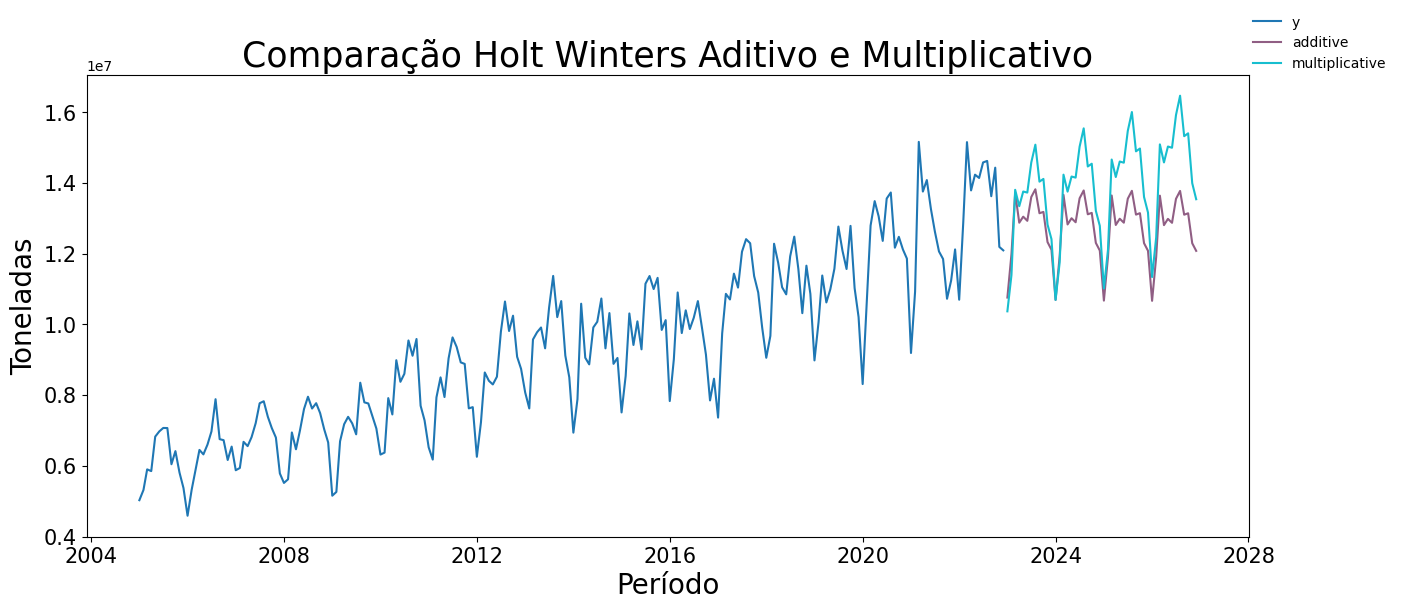
\includegraphics[width=0.85\textwidth]{HW1.png}
\caption{Previsão Holt-Winters Aditivo (modelo que passa nos testes diagnósticos).}
\label{fig:hw}
\end{figure}

\begin{figure}[htb]
\centering
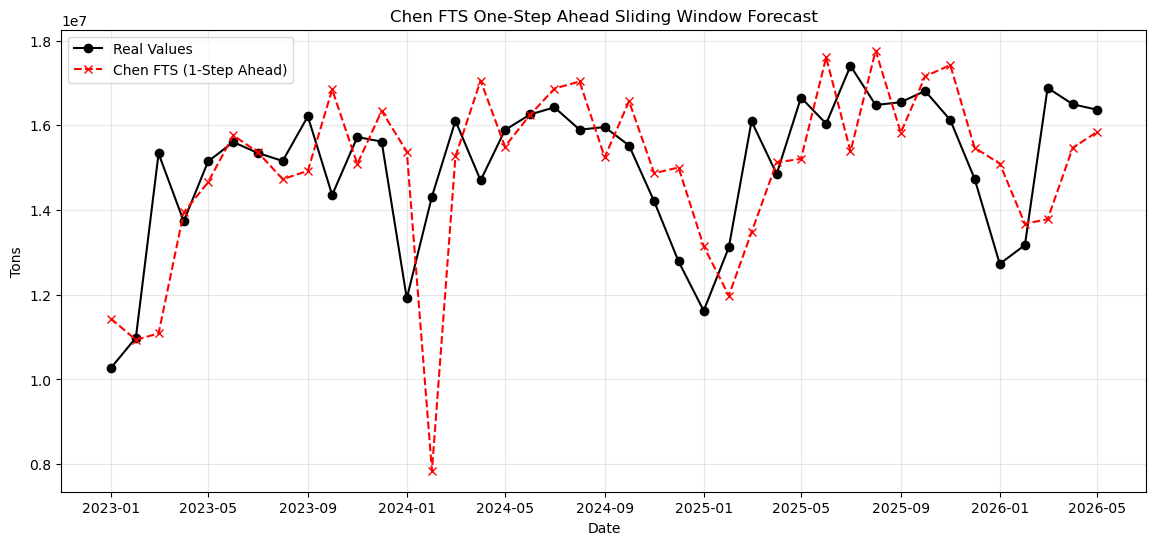
\includegraphics[width=0.85\textwidth]{Chen_SW.png}
\caption{Previsão do modelo Chen FTS sobre $\Delta y$ (\textit{sliding window}).}
\label{fig:chen}
\end{figure}

\begin{figure}[htb]
\centering
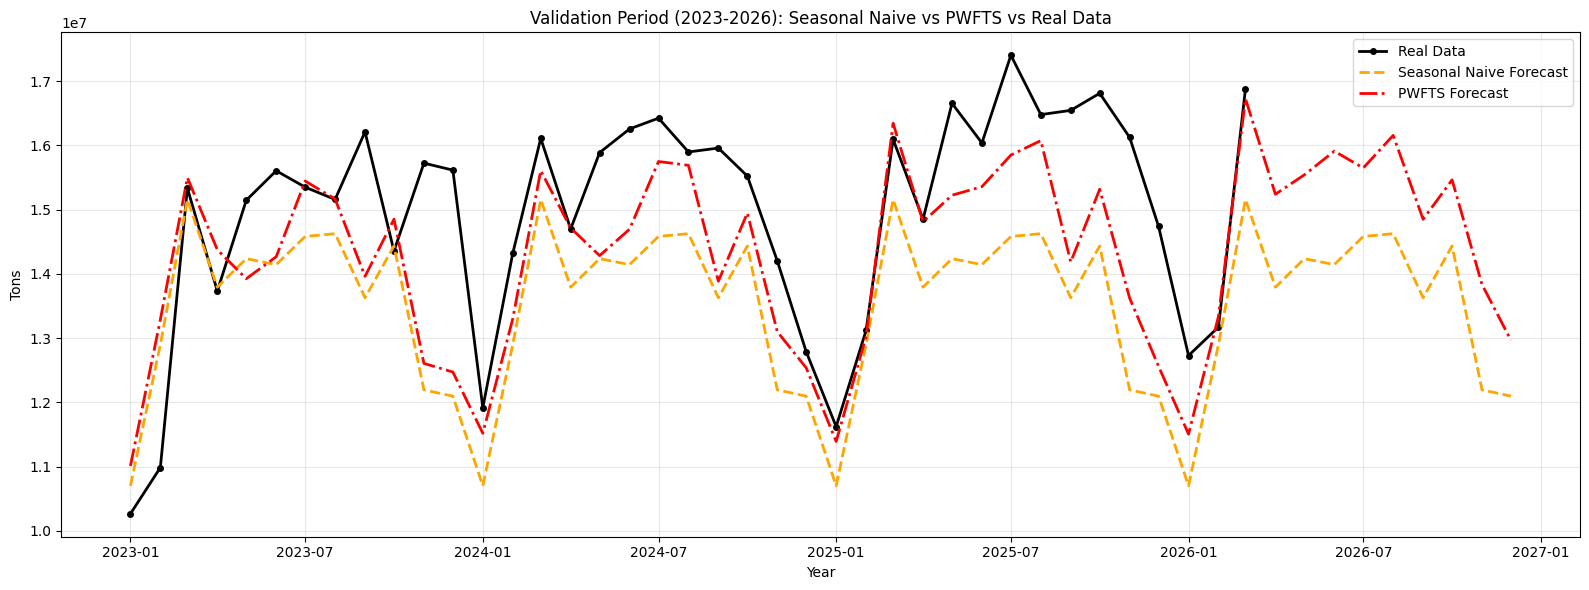
\includegraphics[width=0.85\textwidth]{PWFTS_SNAD.png}
\caption{Previsão PWFTS ($\Delta_{12}y$, ordem 3) comparada ao Sazonal Naïve.}
\label{fig:pwfts}
\end{figure}

A Tabela~\ref{tab:accuracy} apresenta as métricas de acurácia \textit{out-of-sample} dos modelos de previsão avaliados.

\begin{table}[htb]
\centering
\caption{Métricas de acurácia e diagnóstico residual dos modelos avaliados.}
\label{tab:accuracy}
\begin{tabular}{l c c c c l}
\toprule
\textbf{Modelo} & \textbf{Diferenciação} & \textbf{RMSE (ton)} & \textbf{MAPE} & \textbf{LB$_{12}$ ($p$)} & \textbf{Diagnóstico} \\
\midrule
OLS (12 modelos)     & nível   & ---             & ---     & $\approx 0$  & Viola Gauss-Markov \\
Sazonal Naïve        & nível   & 1.863.004       & 10,34\% & $\approx 0$  & Enviesado \\
HW multiplicativo    & nível   & ---             & ---     & $\approx 0$  & Falha LB \\
HW aditivo           & nível   & ---             & ---     & 0,342        & Passa \\
Chen FTS             & $\Delta y$     & 1.835.156 & 9,05\%  & $\approx 0$  & Falha (lags sazonais) \\
\textbf{PWFTS}       & $\Delta_{12}y$ & \textbf{1.503.526} & \textbf{8,21\%} & 0,280 & \textbf{Passa} \\
\bottomrule
\end{tabular}
\end{table}

O PWFTS com diferenciação sazonal e ordem 3 foi o modelo com melhor desempenho tanto em acurácia (RMSE 19,3\% inferior ao Sazonal Naïve; MAPE de 8,21\%) quanto em diagnóstico residual (Ljung-Box com $p > 0{,}25$ em todas as defasagens testadas). O Chen FTS sobre $\Delta y$ obteve MAPE de 9,05\% --- inferior ao Sazonal Naïve (10,34\%) --- mas falhou nos lags sazonais do Ljung-Box, confirmando que a diferença simples não remove sazonalidade.

% ============================================================
\chapter{Discussão e Interpretação dos Resultados}
\label{cap:discussao}
% ============================================================

% ============================================================
\section{Honestidade Axiomática: Definição}
\label{sec:definicao}
% ============================================================

Com base nos resultados obtidos e no referencial teórico articulado, propõe-se a seguinte definição:

\begin{definicao}[Honestidade Axiomática]
\label{def:honestidade}
Um modelo $M$, construído sobre um sistema axiomático $\Sigma$ (uma espécie de estrutura, no sentido de Bourbaki/da Costa/Krause), é \textbf{axiomaticamente honesto} quando nenhuma afirmação inferencial que dele se extrai excede o que suas premissas formais autorizam --- seja porque essas premissas foram testadas e não rejeitadas, seja porque, na ausência de teste, a afirmação foi correspondentemente contida.
\end{definicao}

Essa definição articula dois polos filosóficos: a \textbf{severidade} de \citeonline{mayo2018statistical} (um resultado só é evidência se o procedimento tinha capacidade de detectar a falha) e o \textbf{constrangimento metamatemático} de \citeonline{krause2022models} (todo modelo opera dentro de uma espécie de estrutura cujas premissas delimitam o que pode ser legitimamente afirmado). O pluralismo lógico de \citeonline{dacosta1994sistemas} garante que a escolha do formalismo é livre --- mas o respeito às suas premissas, uma vez feita a escolha, não é opcional.

% ============================================================
\section{Adequação e Honestidade: Eixos Independentes}
\label{sec:eixos}
% ============================================================

O ponto central desta pesquisa é que adequação estatística e honestidade axiomática são critérios \textbf{logicamente independentes}. A Tabela~\ref{tab:grade} ilustra os quatro casos possíveis.

\begin{table}[htb]
\centering
\caption{Grade de adequação $\times$ honestidade, com exemplos.}
\label{tab:grade}
\begin{tabular}{l p{5.5cm} p{5.5cm}}
\toprule
 & \textbf{Honesto} & \textbf{Desonesto} \\
\midrule
\textbf{Adequado}
& Kepler (\citeonline{spanos2007curve}): afirmações conferem com estrutura verificada ($R^2 = 0{,}999$, todos os 5 testes de M-S com $p > 0{,}10$).
& Sobre-extrapolação: afirmação excede o que a adequação licencia (e.g., inferência causal a partir de correlação). \\
\addlinespace
\textbf{Inadequado}
& \textit{Trade-off} informado (\citeonline{nielsen2020practical}): sabe-se que a premissa falha, e a afirmação é escopada de acordo.
& \textbf{Santos et al. (2023)}: afirma ``sucesso'' via $R^2$ sem auditoria --- configura BENT (\citeonline{mayo2018statistical}). \\
\bottomrule
\end{tabular}
\end{table}

Esta grade vale para $\Sigma$ = Kolmogorov-NIID (o sistema axiomático da regressão linear clássica). O modelo de Chen FTS não se encaixa nela diretamente --- opera sob $\Sigma$ distinto (lógica fuzzy), e o eixo ``adequado/inadequado'' análogo simplesmente não foi formalizado para essa arquitetura na literatura consultada. Essa lacuna é, ela mesma, um dos resultados desta pesquisa: a ausência de critério de adequação para FTS na arquitetura de Chen/Song-Chissom é uma pergunta de pesquisa aberta, não uma falha do modelo.

% ============================================================
\section{``Reprovação'' versus ``Abstenção''}
\label{sec:reprovacao}
% ============================================================

Santos et al.\ \textit{reprovaram} num exame que aplicaram tarde demais --- ou nunca aplicaram. O Chen FTS nunca se \textit{inscreveu} nesse exame. A falta de inferência probabilística clássica no OLS de Santos et al.\ é um fracasso \textit{descoberto} via auditoria; no Chen FTS é um fato de \textit{escopo}, por construção da própria lógica fuzzy subjacente. Não são a mesma coisa, e esta pesquisa não as equipara.

Isso esclarece por que a aplicação do teste de Ljung-Box aos resíduos do FTS (Tabela~\ref{tab:ljungbox-all}) não testa \textit{honestidade} --- o FTS nunca afirmou resíduos iid. O que o Ljung-Box mede, nesse contexto, é a \textbf{eficiência informacional residual}: quanto de estrutura temporal ficou sem ser explorada pelo modelo. É uma medida de desempenho, não de integridade axiomática.

% ============================================================
\section{Limitação Apontada em Banca}
\label{sec:limitacao-banca}
% ============================================================

Na apresentação deste trabalho no I Congresso Brasileiro de Filosofia da Ciência (CBFC, 2025), o Prof.\ Júlio Stern (IME-USP) observou que o caso de Santos et al.\ --- doze regressões separadas por mês sobre uma série com tendência e sazonalidade visualmente óbvias --- constitui um alvo ``fácil demais'': a violação seria perceptível por inspeção qualificada, sem necessidade do aparato formal completo. A crítica é procedente e é aqui reconhecida: o caso foi escolhido por sua clareza pedagógica, não por sua severidade como teste do \textit{framework}. A demonstração de que o aparato é \textit{necessário} (e não apenas suficiente) para casos menos óbvios requer auditorias adicionais, indicadas como trabalho futuro.

% ============================================================
\chapter{Conclusões}
\label{cap:conclusoes}
% ============================================================

% ============================================================
\section{O que foi Estabelecido}
\label{sec:estabelecido}
% ============================================================

\begin{enumerate}[label=(\alph*)]
    \item O modelo de regressão linear de \citeonline{santos2023porto} é \textbf{estatisticamente inadequado} --- independência e homocedasticidade são rejeitadas de forma robusta --- e \textbf{axiomaticamente desonesto} --- a afirmação de sucesso via $R^2$ sem auditoria correspondente configura BENT no sentido de \citeonline{mayo2018statistical}.

    \item \textbf{Honestidade axiomática e adequação estatística são critérios logicamente independentes}, não sinônimos. A grade $2 \times 2$ (Tabela~\ref{tab:grade}) demonstra que existem modelos honestos-inadequados e modelos desonestos-adequados.

    \item O modelo de Chen FTS, operando sob axiomas distintos (teoria de conjuntos fuzzy), \textbf{ilustra honestidade axiomática} sem que a pergunta de adequação probabilística sequer se aplique a ele.

    \item A distinção entre paradigmas formais (clássico \textit{vs.}\ fuzzy) não coincide com a distinção entre honestidade e desonestidade: o Holt-Winters multiplicativo (clássico) falha tão catastroficamente quanto a regressão de Santos et al., enquanto o Holt-Winters aditivo (também clássico) e o PWFTS (fuzzy) passam limpo.
\end{enumerate}

% ============================================================
\section{Limitações}
\label{sec:limitacoes}
% ============================================================

\begin{enumerate}
    \item O caso empírico único (Santos et al.) não constitui, sozinho, uma demonstração severa da \textit{necessidade} do aparato filosófico completo --- a violação era detectável por inspeção qualificada, como apontado em apresentação oral (Seção~\ref{sec:limitacao-banca}).

    \item Honestidade axiomática, como definida nesta pesquisa, permanece em nível conceitual --- não é um predicado formal no sentido de Suppes (\textit{Models and Methods in the Philosophy of Science}, Cap.~3), e essa formalização é trabalho futuro.

    \item Não existe, na literatura consultada, um critério de adequação análogo ao de Spanos para modelos de Fuzzy Time Series na arquitetura de Chen/Song-Chissom --- apenas para modelos fuzzy \textit{rule-based} (regressão fuzzy), que possuem estrutura diferente. Construir esse critério é a pergunta de pesquisa que naturalmente sucede esta IC.
\end{enumerate}

% ============================================================
\section{Sugestões para Trabalhos Futuros}
\label{sec:futuros}
% ============================================================

\begin{itemize}
    \item Auditar casos adicionais, publicados em periódicos com revisão por pares, onde a violação de pressupostos não seja visualmente óbvia, fortalecendo o argumento pela severidade do teste.

    \item Investigar o critério de invariância de \citeonline{suppes1993models} (Cap.~3, ``Invariance and Meaningfulness'') como candidato à formalização rigorosa de honestidade axiomática entre sistemas axiomáticos distintos.

    \item Formalizar um critério de adequação específico para FTS na arquitetura de Chen, respondendo à pergunta: existe, para relações lógicas fuzzy, algo estruturalmente equivalente ao teste de Ljung-Box?
\end{itemize}

% ============================================================
% ELEMENTOS PÓS-TEXTUAIS
% ============================================================
\postextual

\bibliography{referencias}

\begin{anexosenv}
    \partanexos
    \chapter{Certificado de Comunicador --- I CBFC}
    \label{an:comunicador}
    Certificado de apresentação de comunicação oral no I Congresso Brasileiro de Filosofia da Ciência (CBFC), 2025.

    \begin{figure}[htb]
    \centering
    
\includegraphics[width=0.9\textwidth]{../I Congresso Brasileiro de Filosofia da Ciência - Certificado de Gabriel Gomes - COMUNICADOR.pdf}
    \caption{Certificado de Comunicador --- I CBFC (2025).}
    \end{figure}

    \chapter{Certificado de Ouvinte --- I CBFC}
    \label{an:ouvinte}
    Certificado de participação como ouvinte no I Congresso Brasileiro de Filosofia da Ciência (CBFC), 2025.

    \begin{figure}[htb]
    \centering
    
\includegraphics[width=0.9\textwidth]{../I Congresso Brasileiro de Filosofia da Ciência - Certificado de Gabriel Gomes - OUVINTE.pdf}
    \caption{Certificado de Ouvinte --- I CBFC (2025).}
    \end{figure}
\end{anexosenv}

\end{document}
